\begin{figure}[h!]
\centering
\caption{Evolución del recaudo del IVA}
\label{fig:vat_rev_rate}
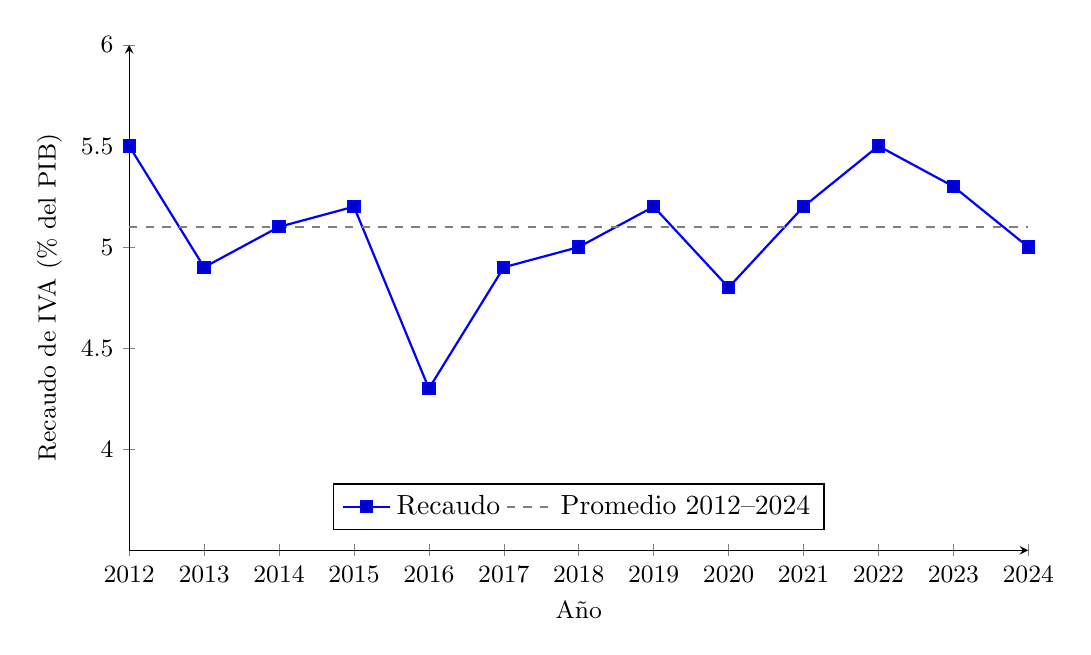
\begin{tikzpicture}
\begin{axis}[
    width=13cm,
    height=8cm,
    xlabel={Año},
    ylabel={Recaudo de IVA (\% del PIB)},
    ymin=3.5, ymax=6,
    ytick={4, 4.5, ..., 6},
    xtick=data,
    xticklabels={%2011,
    2012,2013,2014,2015,2016,2017,2018,2019,2020,2021,2022,2023,2024},
    axis y line=left,
    axis x line=bottom,
    tick label style={font=\small},
    label style={font=\small},
    legend style={at={(0.5,-0.15)}, anchor=north, legend columns=-1},
    every axis plot/.append style={thick},
    legend style={at={(0.5,0.04)}, anchor=south},
]
\addplot+[mark=square*, solid] table[x expr=\coordindex, y=IVA] {
Año IVA
%2011 5.7
2012 5.5
2013 4.9
2014 5.1
2015 5.2
2016 4.3
2017 4.9
2018 5.0
2019 5.2
2020 4.8
2021 5.2
2022 5.5
2023 5.3
2024 5.0
};
\addlegendentry{Recaudo}
% Línea del promedio
\addplot[dashed, thick, gray] coordinates {(0,5.1) (12,5.1)};
\addlegendentry{Promedio 2012–2024}
\end{axis}
\end{tikzpicture}   
\vspace{0.1cm}
\par \footnotesize{Fuente: Balance general del GNC, Ministerio de Hacienda.}
\end{figure}
